\section{\twoMode\ $\SOn{2}$-equivariant flow}
\label{s:twoMode}

Dangelmayr,\rf{Dang86} Armbruster, Guckenheimer and Holmes,\rf{AGHO288}
Jones and Proctor,\rf{JoPro87} and Porter and Knobloch\rf{PoKno05} (see
Golubitsky \etal\rf{golubII}, Sect. XX.1) have investigated bifurcations
in 1:2 resonance ODE normal form models to third order in the amplitudes.
Here, we use this model as a starting point from which we derive what may
be one of the simplest chaotic systems with a continuous symmetry. We refer to this as the {\twomode} system:
\bea
	\dot{z}_1 &=& (\mu_1-\ii\, e_1)\,z_1+a_1\,z_1|z_1|^2
				 +b_1\,z_1|z_2|^2+c_1\,\overline{z}_1\,z_2
	\continue
	\dot{z}_2 &=& (\mu_2-\ii\, e_2)\,{z_2}+a_2\,z_2|z_1|^2
				 +b_2\,z_2|z_2|^2+c_2\,z_1^2 \,,
	\label{eq:DangSO2}
\eea
where $z_1$ and $z_2$ are complex and all parameters real-valued. The parameters $\{e_1,e_2\}$ break the $\On{2}$ symmetry of the
 normal form studied by Dangelmayr\rf{Dang86} leading to an $\SOn{2}$-equivariant
system. As we will show below in \refeq{PKinvEqs1}, only the combination
$(2e_1-e_2)$ matters in the symmetry reduced dynamics, so for simplicity
we set $e_1=0$.\DB{2014-10-28}{We say this and then never really do it in any of the analysis except in numerics. Should we get rid of $e_1$ everywhere or keep it?} This complex two mode system can be expressed as a 4-dimensional
first order real ODE system by substituting $z_1 = x_1 + i\,y_1$, $z_2 = x_2 + i\,y_2$, so that
\bea
\dot{x}_1 &=& (\mu_1 + a_1 r_1^2 + b_1 r_2^2 + c_1 x_2)x_1 + c_1 y_1 y_2 + e_1 y_1 % double checked DBE 05/22/2014
\continue
\dot{y}_1 &=& (\mu_1 + a_1 r_1^2 + b_1 r_2^2 - c_1 x_2)y_1 + c_1 x_1 y_2 - e_1 x_1 % double checked DBE 05/22/2014
\continue
\dot{x}_2 &=& (\mu_2 + a_2 r_1^2 + b_2 r_2^2)x_2 + c_2 (x_1^2 - y_1^2) + e_2 y_2 % double checked DBE 05/22/2014
\label{2mode4D}
\continue
\dot{y}_2 &=& (\mu_2 + a_2 r_1^2 + b_2 r_2^2)y_2 + 2 c_2 x_1 y_1 - e_2 x_2 % double checked DBE 05/22/2014
\continue
		  && \mbox{where } r_1^2 = x_1^2 + y_1^2\, , \quad r_2^2 = x_2^2 + y_2^2
\,.
\eea

This normal form has a large set of parameters $\left(\mu_1,\mu_2,a_1,a_2,b_1,b_2,c_1,c_2,e_1,e_2\right)$.
Following in the tradition of Lorenz\rf{lorenz},
H\'enon\rf{henon} and R\"ossler\rf{ross}, we have played with various
choices of parameters until settling on the following set of values, which we will use in all
numerical calculations presented here:
\beq
	\begin{tabular}{c c c c c c c c c c}
	% after \\: \hline or \cline{col1-col2} \cline{col3-col4} ...
	 $\mu_1$ & $\mu_2$ & $e_1$ & $e_2$ & $a_1$ & $a_2$ & $b_1$ & $b_2$ & $c_1$ & $c_2$ \\
	\hline
	 -2.8	& 1		  & 0	  & 1	  & -1	  & -2.66 & 0	  & 0 	  & -7.75 & 1
	\end{tabular}
	\label{eq:pars}
\eeq
This choice of parameters is far from the bifurcation values studied
by previous authors \rf{Dang86,AGHO288,JoPro87,PoKno05}, so that the
model has no physical interpretation. However, this set of parameters yield chaotic dynamics,
making ours the simplest model for the study of chaotic dynamics in systems with continuous symmetry that we
are aware of: it is a 4\dmn\ $\SOn{2}$-equivariant model in which the three
dimensional $\SOn{2}$-reduced dynamics are chaotic.

It can be checked by inspection that eqs.~\refeq{eq:DangSO2} are
equivariant under the \Un{1}\ transformation
\beq
(z_1,z_2) \rightarrow   (e^{i {\gSpace}}z_1,e^{i 2{\gSpace}} z_2)
\,.
\ee{Dang86(1.1)aa}
In the real representation \refeq{2mode4D}, the $\SOn{2}$ group action
\refeq{Dang86(1.1)aa} is given by $\ssp'= \exp\left( \theta \Lg\right)\ssp$,
where $\transp{\ssp} =$ {\cartpt{x_1, y_1,x_2, y_2}}, and $\Lg$ is the Lie algebra
generator
\beq
\Lg  \, =
\left( \begin{array}{cccc}
         0 & -1 & 0 & 0 \\
         1 & 0 & 0 & 0 \\
         0 & 0 & 0 & -2\\
         0 & 0 & 2 & 0
      \end{array} \right)
\,.
\ee{LGTwoMode}
One can easily check that the real \twomode\ system \refeq{2mode4D}
satisfies the equivariance condition \refeq{inftmInv}.

From \refeq{eq:DangSO2}, it is obvious that the \eqv\ point \((z_1,z_2)=(0,0)\)
is an invariant subspace, and that $z_1=0$, $z_2 \neq 0$ is a 2\dmn\
flow-invariant subspace,
\beq
  \dot{z}_1 = 0 % Double checked DBE 05/26/2014
\,,\qquad
  \dot{z}_2 = (\mu_2-\ii\, e_2 +b_2 |z_2|^2)\,{z_2} % Double checked DBE 05/26/2014
\,,
\ee{eq:DangSO2spsp}
with a single circular \reqv\ of radius $r_2 = \norm{z_2} = \sqrt{-\mu_2/b_2}$ with
\phaseVel\ $\velRel=-e_2/2$. At the origin the stability matrix $\Mvar$ commutes with $\Lg$, 
and thus can be block-diagonalized into two $[2\!\times\!2]$ matrices.
% According to {\bf [2012-04-27 Daniel]},
The eigenvalues of $\Mvar$ at \cartpt{0,0,0,0} are $\Lyap_1 = \mu_1$ with multiplicity 2 and
$\Lyap_2 = \mu_2 \pm i e_2$. The eigenvectors for $\Lyap_1$ are \cartpt{1,0,0,0} and
\cartpt{0,1,0,0} in the \cartpt{x_1,x_2,y_1,y_2} basis. The eigenvectors for $\Lyap_2$
are \cartpt{0,0,1,0} and \cartpt{0,0,0,1}.

In contrast, $z_2 =0$ is not, in general, a flow-invariant subspace, since the dynamics
\[
  \dot{z}_1 = (\mu_1-\ii\, e_1)\,z_1+a_1\,z_1|z_1|^2
\,,\qquad
  \dot{z}_2 = c_2\,z_1^2
\,.
\]
take the flow out of the $z_2 =0$ plane.
    \PC{should we check if anything of interest happens for $c_2 = 0$? }


\subsection{Invariant polynomial bases}
\label{s:invPol}

Consider the \statesp\ of a dynamical system
constructed from two complex Fourier modes\rf{Dang86,AGHO288,PoKno05}
$m=(1,2)$, with the $\SOn{2} \simeq \Un{1}$\DB{2014-10-28}{What does \simeq mean in this context? Aren't they actually the same?} group action given by \refeq{Dang86(1.1)aa}. In this case, it is easy to construct a set of four real-valued
$\SOn{2}$ invariant polynomials
\bea
u &=& {z}_1 \overline{z}_1
    \,,\quad
v = {z}_2 \overline{z}_2
    \continue
w &=& z_1^2 \overline{z}_2 + \overline{z}_1^2 {z}_2
    \,,\quad
q = (z_1^2 \overline{z}_2 - \overline{z}_1^2 {z}_2)/\ii
\,.
\label{Dang86(1.2)PK}
\eea
The polynomials $\{u,v,w,q\}$ are
linearly independent, but related through one syzygy,
\beq
w^2+q^2 - 4\,u^2v = 0 % Double checked syzygy is satisfied by eq Dang86(1.2)PK DBE 05/22/2014
\label{eq:syzPK}
\eeq
that confines the dynamics to a 3-dim\-ens\-ion\-al manifold $\pSRed=\pS/\SOn{2}$, a symmetry-invariant repre\-sent\-ati\-on of the
4-dim\-ens\-ion\-al \SOn{2} equivariant dynamics, which we call the \reducedsp\. By construction, $u \geq
0$, $v \geq 0$, but $w$ and $q$ can be of either sign. That is explicit
in in polar coordinates $ {z}_1 = |u|^{1/2} e^{\ii\phi_1}$, $ {z}_2 =
|v|^{1/2} e^{\ii\phi_2}$, where the  $w, q$ invariants take the form
\bea
w &=& 2\,\Re(z_1^2 \overline{z}_2) = 2\,u |v|^{1/2} \cos \psi %Triple checked DBE 05/22/2014
\continue
q &=& 2\,\Im(z_1^2 \overline{z}_2) = 2\,u |v|^{1/2} \sin \psi %Triple checked DBE 05/22/2014
\,,
\label{Dang86(1.2)polar}
\eea
where $\psi = 2 \phi_1 - \phi_2$.

The dynamical equations for \invpt{u,v,w,q} follow from the chain rule
\( %beq
 \dot{ u}_i= \sum_j ({\partial u_i}/{\partial \ssp_j}) \, \dot{\ssp}_j
 \,,
\) %ee{HilbChainRl}
which yields
\bea
  \dot{u} &=& \overline{z}_1 \dot{z}_1 + {z}_1 \dot{\overline{z}}_1 % Triple checked DBE 05/22/2014
\,,\qquad
  \dot{v} = \overline{z}_2 \dot{z}_2 + {z}_2 \dot{\overline{z}}_2 % Triple checked DBE 05/22/2014
\continue
  \dot{w} &=& 2 \,\overline{z}_2 {z}_1 \dot{z}_1 % Triple checked DBE 05/22/2014
           + 2\,{z}_2 \overline{z}_1 \dot{\overline{z}}_1
           + {z}_1^2 \dot{\overline{z}}_2
           + \overline{z}_1^2 \dot{z}_2
\continue
  \dot{q} &=&  (2\,\overline{z}_2 {z}_1 \dot{z}_1 % Triple checked DBE 05/22/2014
           - 2\,{z}_2 \overline{z}_1 \dot{\overline{z}}_1
           + {z}_1^2 \dot{\overline{z}}_2
           - \overline{z}_1^2 \dot{z}_2
           )/\ii
\label{PKinvEqs}
\eea
Substituting \refeq{eq:DangSO2} into \refeq{PKinvEqs}, we obtain a set
of four $\SOn{2}$-invariant equations,

\bea
  \dot{u} &=& 2\,\mu_1\,u+2\,a_1\,u^2+2\,b_1\,u\,v+c_1\,w % Triple checked DBE 05/22/2014
\continue
  \dot{v} &=& 2\,\mu_2\,v+2\,a_2\,u\,v+2\,b_2\,v^2+c_2\,w % Triple checked DBE 05/22/2014
\continue
  \dot{w} &=& (2\,\mu_1+\mu_2)\,w+(2a_1+a_2)\,u\,w+(2b_1+b_2)\,v\,w % Triple checked DBE 05/22/2014
\ceq
             +\, 4c_1\,u\,v + 2c_2\,u^2 +(2e_1 - e_2)\,q
\label{PKinvEqs1}\\
  \dot{q} &=& (2\mu_1+\mu_2)\,q+(2a_1+a_2)\,u\,q
\ceq
             +(2b_1+b_2)\,v\,q
             -(2e_1-e_2)\,w % Triple checked DBE 05/22/2014
\,.
\nnu
\eea
Note that the $\On{2}$-symmetry breaking parameters
 $\{e_1,e_2\}$ of the
Dangelmayr normal form system\rf{Dang86} appear only in the
relative phase combination $(2e_1-e_2)$.
%[2012-07-31 Evangelos]
Using the syzygy \refeq{eq:syzPK}, we can
eliminate $q$ from \refeq{PKinvEqs1} to get
    \PC{
    Note that $4u^2v-w^2 = 4u^2v(1-\cos^2\psi)$, so
    no serious singularity is introduced this way. Perhaps
    write equations of $(u,v,\cos \psi)$ as in the
    ChaosBook exercises?
    }
\bea
  \dot{u} &=& 2\,\mu_1\,u+2\,a_1\,u^2+2\,b_1\,u\,v+c_1\,w \nonumber % Triple checked DBE 05/22/2014
\\
  \dot{v} &=& 2\,\mu_2\,v+2\,a_2\,u\,v+2\,b_2\,v^2+c_2\,w \label{PKinvEqs1syz}  % Triple checked DBE 05/22/2014
\\
  \dot{w} &=& (2\,\mu_1+\mu_2)\,w+(2a_1+a_2)\,u\,w+(2b_1+b_2)\,v\,w % Triple checked DBE 05/22/2014
\ceq
             +\, 4c_1\,u\,v + 2c_2\,u^2 +(2e_1 - e_2)(4u^2v-w^2)^{1/2}\,
  \nonumber
\eea

This invariant basis can be used either to investigate the dynamics directly or 
to visualize solutions\rf{GL-Gil07b} computed in the full equivariant basis \refeq{eq:DangSO2}. 
While representations of our model in terms of invariant polynomials \refeq{PKinvEqs1}
and polar coordinates \refeq{Dang86(1.2)polar} are useful for cross-checking calculations in the 
full \statesp\ $\transp{\ssp} =$ \cartpt{x_1, x_2,y_1, y_2}, construction requires a bit of algebra
even for this simple 4-dimensional flow. For very high\dmn\ flows, such as \KS\ and \NS\ flows, we 
do not know how to carry out such constructions.

\subsubsection{\Eqva\ of the symmetry-reduced dynamics}
\label{s:eqva}

The first step in elucidating the geometry of attracting
sets is the determination of their \eqva. We shall now show that the problem of determining
the \eqva\ of the symmetry-reduced \twomode\ \refeq{PKinvEqs1} system \invpt{u^*,v^*,w^*,q^*} can be reduced to finding the roots of a multinomial expression.\ES{2014-05-15}{Why do you count complex
solutions as equilibria?}
%[2012-04-28 Predrag]
First, let we define
\beq
A_1= \mu_1+a_1\,u+b_1\,v
    \,,\qquad
A_2 = \mu_2+a_2\,u+b_2\,v
\ee{PKinvEqs2a}
and rewrite \refeq{PKinvEqs1} as
%     \newpage
\bea
  0  &=&  2\,A_1\,u +c_1\,w % Double checked DBE 05/24/2014
    \,,\qquad
  0  =  2\,A_2\,v +c_2\,w % Double checked DBE 05/24/2014
\continue
  0  &=& (2\,A_1+ A_2)\,w
          +2\,\left(c_2\,u+2\,c_1\,v\right)\,u % Double checked DBE 05/24/2014
          \ceq
		  + (2e_1-e_2)\,q
\label{PKinvEqs3}\\
  0  &=& (2\,A_1+ A_2)\,q - (2e_1-e_2)\,\,w % Double checked DBE 05/24/2014
\nnu
\eea
We already know that \invpt{0,0,0,0} and \invpt{0,-\mu_2/b_2,0,0} are roots are the only roots in the 
$u=0$ and $v=0$ subspaces, so we are looking only for the $u>0$, $v>0$, $w,q \in \reals$ solutions; 
there could be problems\ES{2014-05-15}{What problems?}\DB{2014-10-29}{Also not sure what the problem is... Do we remember?} 
from the non-generic roots with either $w=0$ or $q=0$, but not both
simultaneously, since the syzygy \refeq{eq:syzPK} precludes that. Either $w$ or $q$
can be eliminated by obtaining the following relations from \refeq{PKinvEqs3}:
\bea
	w  &=& - \frac{2\,u}{c_1}\,A_1 = - \frac{2\,v}{c_2}\,A_2 % Double checked DBE 05/24/2014
	\continue
	q &=& \frac{2(-2e_1+\,e_2)\,u\,v}{c_2\,u+2\,c_1\,v} . % Having issues with this DBE 05/24/2014... potentially drops a w = 0 root.
	\label{PKinvEqs4}
\eea
Substituting \refeq{PKinvEqs4}\DB{}{I think getting to the equation for $q$ throws out a potential $w = 0$ root. Do the first two equations then imply that u,v = 0? If, so then q = 0 and there's no problem, but I don't think that's the most general case.} into \refeq{PKinvEqs3} we get two bivariate
polynomials whose roots are the \eqva\ of the system \refeq{PKinvEqs1}:
\bea
	f(u,v) &=& c_2\,u\,A_1 - c_1\,v\,A_2 = 0 \,,\qquad  \nonumber
	\\
	g(u,v) &=&
 \left(4\,A_1^2 u^2 - 4\,c_1^2\,u^2 v\right)\left(c_2\,u+2\,c_1\,v\right)^2 \label{PKinvEqs5} %Double checked DB 04-30-2012
	\ceq
	+\,4\,c_1^2\,(-2e_1+e_2)^2\,u^2\,v^2 = 0
\,,
	\\
	deg(f) &=& 2, \, deg(g) = 6 \nonumber
\,.
\eea
%\DBedit{DB: Not sure where this factor of 2 comes from in $w =
%-\frac{2}{e_2} (2\,A_1+ A_2)\,q $. From the last equation in
%\refeq{PKinvEqs3}, I get $w = -\frac{1}{e_2} (2\,A_1+ A_2)\,q$.
%Therefore, I get I get  $q = \frac{2 e_2\,u\,v}{c_2\,u+2\,c_1\,v}$}
%2012-04-29 Predrag: thanks!

% \DBedit{DB: I get $g(u,v) = \left(w^2 - 4\,u^2
% v\right)\left(c_2\,u+2\,c_1\,v\right)^2 +\,4\,e_2^2\,u^2\,v^2 = 0$}
%2012-04-29 Predrag: thanks!
%2012-04-29 Predrag: should have I used the syzygy \refeq{eq:syzPK},
%$w^2 - 4\,u^2v = -q^2$ DB: If you plug the syzygy in you trivially get zero....

We divide the common multiplier $u^2$ from the second equation and by
doing so, eliminate one of the two roots at the origin, as well as the
\cartpt{0,-\mu_2/b_2,0,0} root within the invariant subspace
\refeq{eq:DangSO2spsp}. Furthermore, we scale the parameters and
variables as
$\tilde{u} = c_2\,u$,
$\tilde{v} = c_1\,v$,
$\tilde{a_1} = a_1/c_2$,
$\tilde{b_1} = b_1/c_1$,
$\tilde{a_2} = a_2/c_2$,
$\tilde{b_2} = b_2/c_1$ 
to get
\bea
\tilde{f}(\tilde{u},\tilde{v}) &=&
  \tilde{u}\,\tilde{A}_1 - \tilde{v}\,\tilde{A}_2 = 0 %Double checked DB 04-30-2012
\,,\qquad deg(f) = 2 \label{PKinvEqs5a}
\\
\tilde{g}(\tilde{u},\tilde{v}) &=&  %Double checked DB 04-30-2012
 \left(\tilde{A}_1^2
 - c_1\,\tilde{v}\right)
 \left(\tilde{u}+2\,\tilde{v}\right)^2
 +e_2^2\,\tilde{v}^2 = 0
\,,
\ceq
   deg(g) = 4 \label{PKinvEqs5b}
\\
 && \mbox{where }
\tilde{A}_1 = \mu_1+\tilde{a_1}\,\tilde{u}+\tilde{b_1}\,\tilde{v}
\,,\ceq
\qquad\quad \tilde{A}_2 = \mu_2+\tilde{a_2}\,\tilde{u}+\tilde{b_2}\,\tilde{v}
\,,
\label{PKinvEqs5c}
\eea

Solving coupled bivariate polynomials \refeq{PKinvEqs5a} is not, in general, a trivial task. However,
for the choice of parameters given by \refeq{eq:pars}, eq.~\refeq{PKinvEqs5a} yields
$\tilde{v} = (\mu_1 + \tilde{a}_1 \tilde{u})/(\mu_2 + \tilde{a}_2
\tilde{u})$. Substituting this into \refeq{PKinvEqs5b} makes it a fourth order polynomial in $u$, 
which we can solve. Only non-negative, real roots of this polynomial have a correspondence in the \twomode\
\statesp\ since $u$ and $v$ are the squares of first and second mode amplitudes,
respectively. Two roots satisfy this condition, the \eqv\ at the origin:
\beq
	\invpol_{\EQV{}} = (0,0,0,0)\,, %\qquad \mbox{(double)}
\ee{eq:origin}
and the \reqv :
\beq
	\invpol_{\REQV{}{}} = (0.193569,0.154131,-0.149539,-0.027178)\,.
\ee{eq:reqv}
Note that by setting $b_2 = 0$, we send the \reqv\ at $\invpol =
(0,-\mu_2/b_2,0,0)$ to infinity. Thus, \refeq{eq:reqv} is the only \reqv\
of the \twomode\ system for our choice of parameters. While this is an equilibrium
in the invariant polynomial basis, in the \SOn{2}-equivariant, real-valued
\statesp this is a \reqv\ and traces out its group orbit. A representative point on this orbit is:
\[
  \left(x_1, y_1, x_2, y_2\right) = \left(0.439966, 0, -0.386267, 0.070204\right) .
\]


\subsubsection{No chaos when the reflection symmetry is restored}
\label{s:dfsafs}

Before finishing our discussion of invariant polynomials, we make an
important observation regarding the case when both of the reflection symmetry breaking
parameters, $e_{1}$ and $e_2$ are set to $0$. In this case, $\sspC_{1,2} \rightarrow \bar{\sspC}_{1,2}$ 
symmetry is restored and the evolution equations for $u$, $v$, and $w$ in \refeq{PKinvEqs1} become 
independent of $q$. Furthermore, the time evolution equation for $q$ becomes linear in $q$ itself, so that 
it can be expressed as:
\beq
    \dot{q} = \xi (u, v) q \,.
\ee{e-qlinearq}
Hence, the time evolution of $q$ can be written as
\beq
    q(\zeit) =  e^{\int_0^\zeit d \zeit' \xi (u(\zeit'), v(\zeit'))} q(0) \, .
\ee{e-qO2solq}
If we assume that the flow is bounded, then we can also assume that a long time
average of $\xi$ exists. The sign of this average determines the long term
behavior of $q(\zeit)$; it will either diverge or vanish depending on the sign of
$\langle \xi \rangle$ being positive or negative respectively. The former case
leads to a contradiction: If $q(\zeit)$ diverges, the symmetry-invariant flow cannot
be bounded since the syzygy \refeq{eq:syzPK} must be satisfied at all times. If
$q(t)$ vanishes, there are three invariant polynomials left, which are still
related to each other by the syzygy. Thus, the flow is confined
to a two dimensional manifold and cannot exhibit chaos. This is a result holds\DB{2014-11-03}{Do we know
that it holds ONLY in this case? Or do we just not know if it holds in other cases?}
for two mode truncations of the equivariant normal form with terms up to third order.

\subsection{Visualizing \twomode\ dynamics}
\label{s:visual}

\begin{figure*}%[H]
\centering
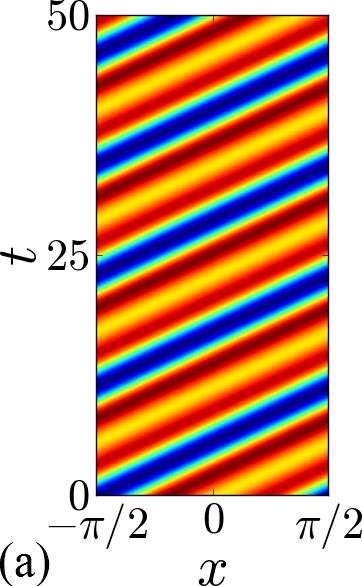
\includegraphics[height=0.22\textwidth]{2modes-conf-reqv}\quad%
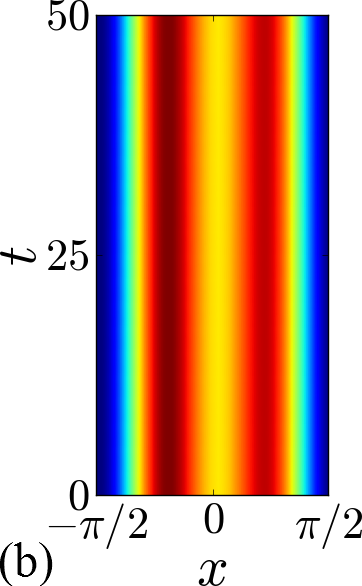
\includegraphics[height=0.22\textwidth]{2modes-confred-reqv}\quad%
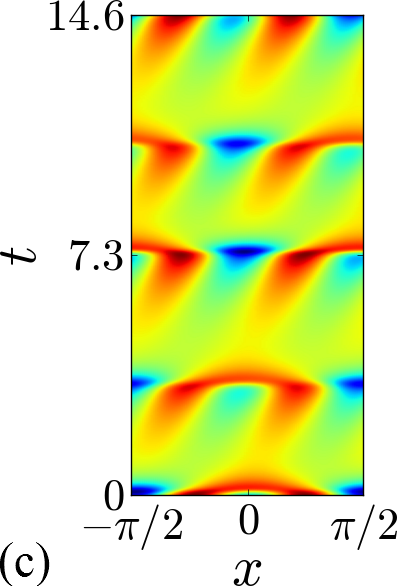
\includegraphics[height=0.22\textwidth]{2modes-conf-rpo}\quad%
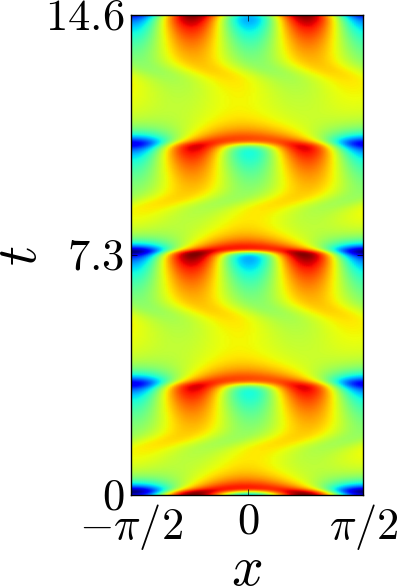
\includegraphics[height=0.22\textwidth]{2modes-confred-rpo}\quad%
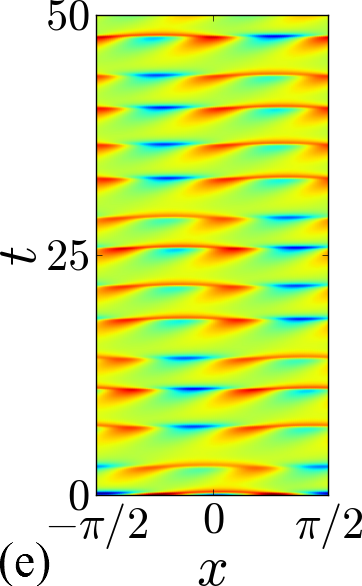
\includegraphics[height=0.22\textwidth]{2modes-conf-ergodic}\quad%
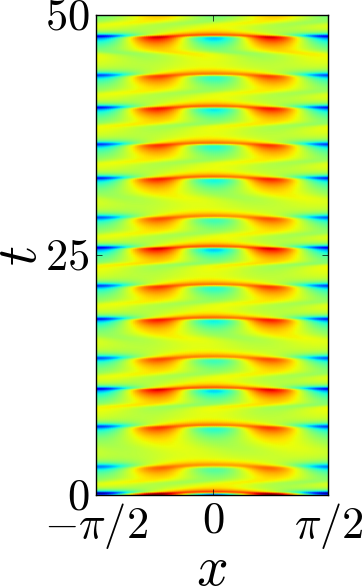
\includegraphics[height=0.22\textwidth]{2modes-confred-ergodic}%
\caption{(Color online)
The \reqv\ \REQV{}{} in
 (a) the system's configuration space becomes an \eqv\ in
 (b) the symmetry-reduced configuration space.
Two cycles of the \rpo\ \cycle{01} in the
 (c) the symmetry-equivariant configuration space become a \po\ in
 (d) the symmetry-reduced configuration space.
A typical ergodic trajectory of the \twomode\ system
in the system's configuration space (e),
 in the symmetry-reduced configuration space (f).
The color scale used in each figure is different to enhance contrast.
}
\label{fig:2modes-conf}
\end{figure*}

\begin{figure*}%[H]
\centering
(a)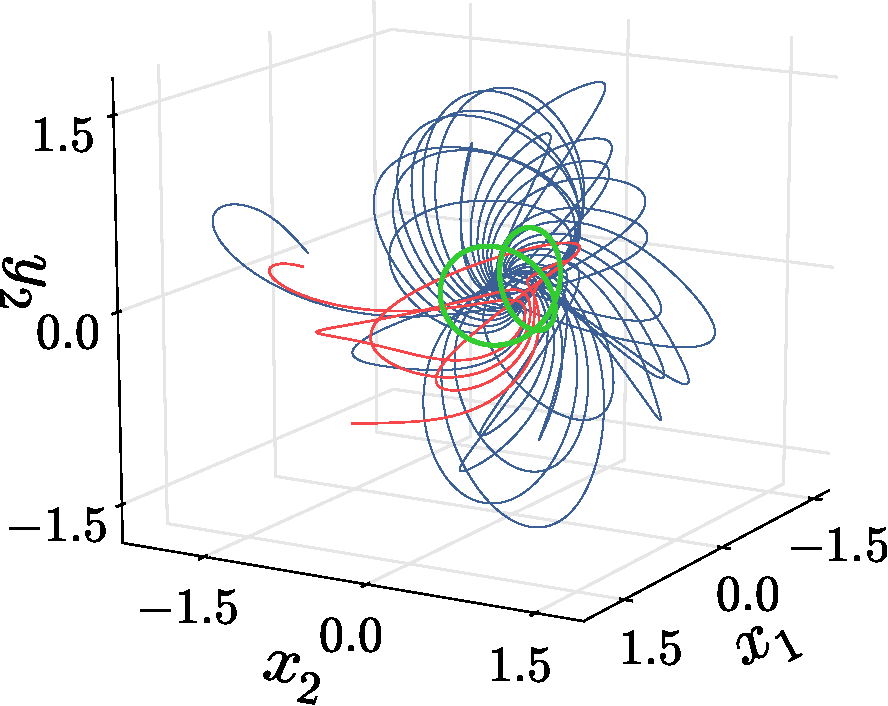
\includegraphics[width=0.30\textwidth]{2modes-ssp}
(b)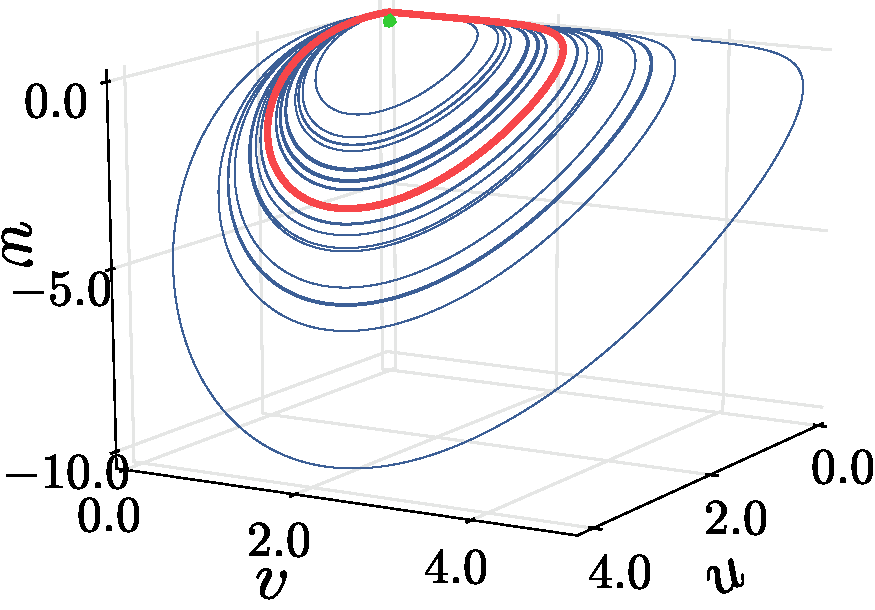
\includegraphics[width=0.30\textwidth]{2modes-invpol}
(c)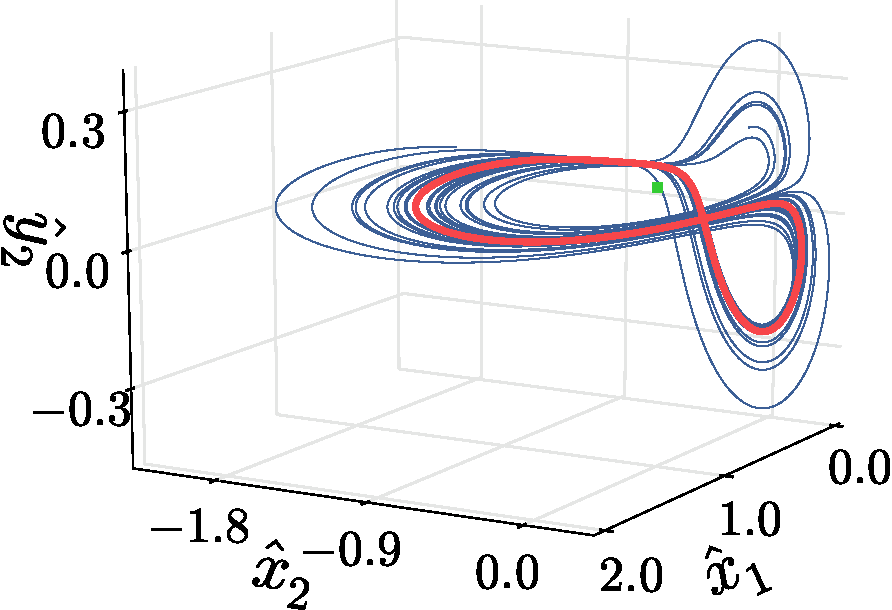
\includegraphics[width=0.30\textwidth]{2modes-sspRed}
\caption{(Color online)
The same trajectories as in \reffig{fig:2modes-conf} (a), (c), and (d),
colored green, red and blue respectively,
	(a) in a 3D projection of the 4\dmn\ \statesp ,
	(b) in a terms of 3 invariant polynomials,
	(c) in the 3\dmn\  first Fourier mode \slicePlane.
Note that in the symmetry reduced representations (b and c), the \reqv\ \REQV{}{}
is reduced to an \eqv , the green point; and the \cycle{01} (red) closes onto
itself after one repeat. In contrast to the invariant polynomial representation (b),
in the first Fourier mode \slicePlane (c), the qualitative difference between shifts
by $\approx \pi$ and $\approx-\pi$ in near passages to the {\sliceBord} is very clear,
and it leads to the unimodal Poincar\'e return map of \reffig{fig:psectandretmap}.
}
\label{fig:2modes-ssp}
\end{figure*}

We now present visualizations of the dynamics of the \twomode\ system in four different
representations: as 3D projections of the four-dimensional real-valued
\statesp, as 3D projections in the invariant polynomial basis, as dynamics in the 3D \slicePlane, and as
two-dimensional spacetime diagrams of the color-coded field $u(\conf,\zeit)$\DB{11-3-2014}{Using $u$ here 
is confusing since we've just spent the last few pages talking about $u$ in the $(u,v,w,q)$ basis}
is defined as follows:
\bea
	u(\conf, \tau) &=& \sum_{k=-2}^{2} \sspC_k(\zeit) e^{i k \conf}\, ,
	\continue && \mbox{where} \, \sspC_{-k} = \bar{\sspC_k} \, , \,
	\sspC_0 = 0\, , \continue && \mbox{and} \, \conf \in [- \pi, \pi]
\, .
\eea
We can also define the symmetry reduced configuration space representation
as the inverse Fourier transform of the symmetry reduced Fourier modes:
\bea
	\hat{u}(\conf, \tau) &=& \sum_{k=-2}^{2} \sspRedC_k(\zeit) e^{i k \conf}\, ,
	\continue && \mbox{where} \, \sspRedC_{-k} = \bar{\sspRedC_k} \, , \,
	\sspRedC_0 = 0\, , \continue && \mbox{and} \, \conf \in [- \pi, \pi]
\, .
\eea
\refFig{fig:2modes-conf}(a) and \ref{fig:2modes-conf}(b) show the sole \reqv\ \REQV{}{}
of the \twomode\ system in the symmetry-equivariant and symmetry-reduced
configuration spaces, respectively. After
the symmetry reduction, the \reqv\ becomes an \eqv . \refFig{fig:2modes-conf}(c) and \ref{{fig:2modes-conf}}(d) show the
\rpo\ \cycle{01} again respectively in the symmetry-equivariant and
symmetry-reduced configuration space representations. Similar to the
\reqv, the \rpo\ becomes a \po\ after symmetry reduction. Finally,
\refFig{fig:2modes-conf}(e) and \ref{fig:2modes-conf}(d) show a typical ergodic trajectory
of the \twomode\ system in symmetry-equivariant and symmetry-reduced
configuration space representations. Note that in each case, symmetry
reduction cancels the `drifts' along the symmetry ($x$) direction.

As can be seen clearly in \reffig{fig:2modes-ssp}(a), these drifts show up in 
the Fourier mode representation as $\SOn{2}$ rotations. The \reqv\ \REQV{}{} 
traces its \SOn{2} group orbit (green curve in \reffig{fig:2modes-ssp} (a)) 
as it drifts in the configuration space. The
\rpo\ \cycle{01} (red) and the ergodic trajectory (blue) rotate
in the same fashion as they evolve. \refFig{fig:2modes-ssp} (b) and \ref{fig:2modes-ssp}(c)
show a three dimensional projection onto the invariant polynomial basis and the 3\dmn\ 
trajectory on the \slicePlane\ for the same orbits. In both figures, the \reqv\ is reduced
to an \eqv\ and the \rpo\ is reduced to a \po.
